\documentclass[10pt,letterpaper]{article}

\usepackage{cogsci}
\usepackage{pslatex}
\usepackage[nodoi]{apacite}
\usepackage{graphicx}
\usepackage[american]{babel}
\usepackage{amsmath}
\usepackage[section]{placeins}
\usepackage{enumitem}
\usepackage{tikz}
\usetikzlibrary{bayesnet}

\title{Linguistic input is coordinated to children's developmental level}
 
 \author{{\large \bf Daniel Yurovsky} \\ \texttt{yurovsky@stanford.edu}\\ Department of Psychology \\ Stanford University
 	\And {\large \bf Gabriel Doyle} \\ \texttt{gdoyle@stanford.edu} \\ Department of Psychology \\ University of California,\\ San Diego
	\And {\large \bf Michael C. Frank} \\ \texttt{mcfrank@stanford.edu} \\ Department of Psychology \\ Stanford University}

\begin{document}

\maketitle

\begin{abstract}


\textbf{Keywords:} 
Language acquisition, word learning, categorization, cognitive development
\end{abstract}

\section{Introduction}

Children learn a tremendous amount about language in their first few years of life. By the time they are able to run down the street, typically developing children have over a thousand words in their productive vocabularies \cite{mayor2011}. They can combine these words to produce new, meaningful multi-word utterances \cite{lieven2009}. They can even use this this budding knowledge to learn new words from just the syntactic constructions in which they occur \cite{yuan2009}.

What explains this rapid acquisition? The last two decades of research have uncovered an abundance of surprising competencies in very young children. For instance, children as young as 6-months-old can use a speaker's gaze as a cue to her intended referent \cite{dentremont1997, senju2008}. By 8-months children can use distributional properties of language to segment discrete words from continuous speech \cite{saffran1996}, and by 12-months can use these same kinds of cues to learn ordering regularities in artificial grammars \cite{gomez1999} and mappings between words and objects \cite{smith2008}. 

However, while these and other competencies are available early, children's \emph{performance} in these domains can be significantly lower. For instance, the abilities to rapidly follow a speaker's gaze---and to subsequently use this disambiguating information to learn a new word---improves dramatically over the first 4 years \cite{yurovsky2016}. Similarly, children's learning of new words from distributional properties of language is highly constrained by their developing attentional and memory systems \cite{frank2011, vlach2012, vlach2013}.

Why is language acquisition so fast if infant learners are so constrained? One possibility is that these tasks designed to target the learning mechanisms available to young children remove cues for learning available in real language input. Indeed, children appear to show significantly higher learning performance when redundant cues to learning available \cite<e.g.,>{frank2009, thiessen2009, shukla2011}. Child-directed input---across a variety of levels and structures---appears to contain many of these kinds of cues, and to facilitate learning \cite{gogate2000, thiessen2005, yurovsky2012}.

However, closer scrutiny in specific domains sometimes yields surprising puzzles. For instance, prosodic properties of child-directed speech are believed to be beneficial for learning phonological acquisition \cite{fernald1989, kuhl1997}. However, recent work suggests that some of the properties may make learning adult-like vowels \emph{hard} \cite{mcmurray2013}. Similarly, child-directed speech typically contains simpler and less variable syntactic structures. This simplicity is thought to aid in early grammatical acquisition, but also makes it \emph{harder} to learn more complex constructions \cite{montag2015a, montag2015b}.

The solution to these puzzles is to consider that these learning processes all unfold over development: The learning problem faced by 6-month-olds is different from the learning problem faced by 2-year-olds, and similarly the learning capacities of a 6-month-old are different from those of a 2-year-old. We propose that the explanation for rapid language acquisition lies neither in the child's early competence, nor in the structure of the input alone; language learning emerges from the  \emph{coordination} between children's developing competencies and the input their caregivers provide \cite{vygotsky1978}. 

If this hypothesis is correct, child-directed speech should be neither uniformly helpful nor uniformly harmful---child directed speech itself should not be uniform. Instead, the structure of linguistic input should be non-stationary, changing as children develop, learn, and become more competent speakers themselves \cite{elman1993, fausey2016}. This is because child-directed speech is not an independent property of the world---it as an action taken by caregivers to communicate with their children. To communicate successfully, caregivers must be mindful of the cognitive and linguistic capacities of their children, and tailor their speech accordingly. 

We test this hypothesis using \emph{linguistic alignment}, a measure of how much speakers change what they say based on what their conversational partners say. We predict that caregivers should align more to their younger children, altering their speech more when children need more linguistic support. In contrast, we predict that children should increase their alignment across development, as they become more competent conversational partners.

\subsection{Linguistic alignment}

When we use language to communicate, we are trying to use the words we say to convey the message we intend. Some of the words will be obligatory to getting the message across: If I want to tell you that we are having sweet potatoes for dinner, I have little choice but to use the words ``sweet potato.'' However, many of the words are optional, and their inclusion or omission has less effect on the message (e.g. ``We [should have/are having] [some/those] sweet potatoes for dinner.''). 

Speakers make these choices for a variety of reasons---from low-level reasons like difficulties of co-articulation to high-level reasons like regional dialects. We focus here one particular reason for these choices: contingency on their conversational partner. In particular, when we talk, we will become more likely to use each-other's expressions, aligning to each other. This kind of alignment appears to be a pervasive property of human social interaction and linguistic communication \cite{giles1991}. 
Further, this alignment appears to be useful, facilitating fluent processing of speech, and increasing the probability of successful communication and accomplishment of joint goals \cite{ireland2011, fusaroli2012}. Critically, alignment is directional: even in the same contexts, some speakers will align more than others. For instance, alignment varies across a social hierarchy, with less powerful speakers aligning more to powerful speakers \cite{kacewicz2013}. Thus, linguistic alignment can measure how much a speaker's choice of words reflects an effort to coordinate to a conversational partner. We leverage this property to measure the extent to which parents are altering the way the speak to coordinate with their developing children.

\section{Model}

\begin{table}
\begin{tabular}{r p{.35\textwidth}}
\hline
Naima: & Eating \textbf{that}. Eating \textbf{some of that}.\\

Mom: & \textbf{Some of this}? \textbf{You} know what \textbf{that is}? \textbf{It is} sweet potato.\\

Naima: & \textbf{I} am \textbf{a} bear \textbf{that} eats.\\

Mom: & \textbf{You're a} bear \textbf{that} eats what? What do \textbf{you} eat little bear?\\
\hline
\end{tabular}
\label{tab:naima}
\caption{Sample parent-child interaction. Bolded words were included in the alignment model.}
\end{table}



Model stuff here. 

\begin{figure*}[t]
  \begin{center}
    % model_lda.tex
%
% Copyright (C) 2010,2011 Laura Dietz
% Copyright (C) 2012 Jaakko Luttinen
%
% This file may be distributed and/or modified
%
% 1. under the LaTeX Project Public License and/or
% 2. under the GNU General Public License.
%
% See the files LICENSE_LPPL and LICENSE_GPL for more details.

% Latent Diriclet allocation model

%\beginpgfgraphicnamed{model-lda}
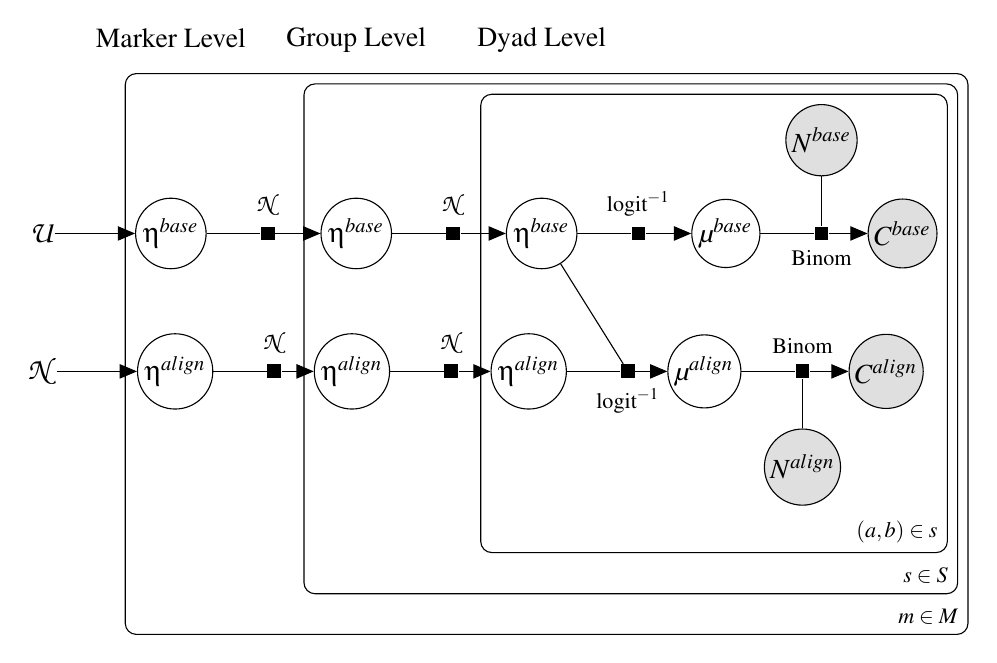
\begin{tikzpicture}[x=1.7cm,y=1.8cm]

  % Nodes

  \node[const] (base) {$\mathcal{U}$};
%  \node[latent,right=.6 of base] (n_b_m) {$\eta^{base}_m$}; 
%  \node[latent,right=.8 of n_b_m] (n_b_ms) {$\eta^{base}_{m,s}$};
%  \node[latent,right=.8 of n_b_ms] (n_b_mab) {$\eta^{base}_{m,a,b}$};
%  \node[latent,right=.8 of n_b_mab] (m_b_mab) {$\mu^{base}_{m,a,b}$};
%  \node[obs,right=.8 of m_b_mab] (C_b_mab) {$C^{base}_{m,a,b}$};

  \node[const,below=.8 of base] (align) {$\mathcal{N}$};
% \node[latent,right=.6 of align] (n_a_m) {$\eta^{align}_m$}; 
% \node[latent,right=.75 of n_a_m] (n_a_ms) {$\eta^{align}_{m,s}$};
% \node[latent,right=.75 of n_a_ms] (n_a_mab) {$\eta^{align}_{m,a,b}$};
% \node[latent,right=.75 of n_a_mab] (m_a_mab) {$\mu^{align}_{m,a,b}$};
% \node[obs,right=.8 of m_a_mab] (C_a_mab) {$C^{align}_{m,a,b}$};

  \node[latent,right=.6 of base] (n_b_m) {$\eta^{base}$}; 
  \node[latent,right=.85 of n_b_m] (n_b_ms) {$\eta^{base}$};
  \node[latent,right=.85 of n_b_ms] (n_b_mab) {$\eta^{base}$};
  \node[latent,right=.85 of n_b_mab] (m_b_mab) {$\mu^{base}$};
  \node[obs,right=.8 of m_b_mab] (C_b_mab) {$C^{base}$};

  \node[latent,right=.6 of align] (n_a_m) {$\eta^{align}$}; 
  \node[latent,right=.75 of n_a_m] (n_a_ms) {$\eta^{align}$};
  \node[latent,right=.75 of n_a_ms] (n_a_mab) {$\eta^{align}$};
  \node[latent,right=.75 of n_a_mab] (m_a_mab) {$\mu^{align}$};
  \node[obs,right=.8 of m_a_mab] (C_a_mab) {$C^{align}$};

  
  \node[const,above=1.05 of n_b_m] (marker) {Marker Level};
  \node[const,above=1.02 of n_b_ms] (group) {Group Level};
  \node[const,above=1.02 of n_b_mab] (dyad) {Dyad Level};

  % Factors
  
  \factor[right=of n_b_m] {n_b_m_f} {above:$\mathcal{N}$} {} {};
  \factor[right=of n_b_ms] {n_b_ms_f} {above:$\mathcal{N}$} {} {};
  \factor[right=of n_b_mab] {n_b_mab_f} {above:$\textrm{logit}^{-1}$} {} {};
  \factor[right=of m_b_mab] {m_b_mab_f} {below:Binom} {} {};

  \factor[right=of n_a_m] {n_a_m_f} {above:$\mathcal{N}$} {} {};
  \factor[right=of n_a_ms] {n_a_ms_f} {above:$\mathcal{N}$} {} {};
  \factor[right=of n_a_mab] {n_a_mab_f} {below:$\textrm{logit}^{-1}$} {} {};
  \factor[right=of m_a_mab] {m_a_mab_f} {above:Binom} {} {};

  %\factor[right=of C_b_mab] {C_b_mab_f} {above:Binom$} {} {};
  
  %\factor[above=of X]     {X-f}     {Multi} {} {} ; %
  %\factor[above=of T]     {T-f}     {left:Multi} {} {} ; %
  %\factor[above=of theta] {theta-f} {left:Dir} {} {} ; %

  % More nodes
  %\node[latent, right=of X-f] (phi)  {$\phi$}; %
  %\node[const, above=of phi]  (aphi) {$\alpha_\phi$}; %

  %\factor[above=of phi] {phi-f} {right:Dir} {} {} ; %

%  \node[obs,above=.35 of m_b_mab_f] (N_b_mab) {$N^{base}_{m,a,b}$};
%  \node[obs,below=.35 of m_a_mab_f] (N_a_mab) {$N^{align}_{m,a,b}$};

  \node[obs,above=.35 of m_b_mab_f] (N_b_mab) {$N^{base}$};
  \node[obs,below=.35 of m_a_mab_f] (N_a_mab) {$N^{align}$};


  \edge{base}{n_b_m};
  \factoredge {n_b_m}  {n_b_m_f}     {n_b_ms} ; %
  \factoredge {n_b_ms}  {n_b_ms_f}     {n_b_mab} ; %
  \factoredge {n_b_mab}  {n_b_mab_f}     {m_b_mab} ; %
  \factoredge {m_b_mab,N_b_mab} {m_b_mab_f} {C_b_mab}; %
 
   \edge{align}{n_a_m};
  \factoredge {n_a_m}  {n_a_m_f}     {n_a_ms} ; %
  \factoredge {n_a_ms}  {n_a_ms_f}     {n_a_mab} ; %
  \factoredge {n_a_mab,n_b_mab}  {n_a_mab_f}     {m_a_mab} ; %
  \factoredge {m_a_mab,N_a_mab} {m_a_mab_f} {C_a_mab}; %
 %\factoredge {atheta} {theta-f} {theta} ; %
  %\factoredge {phi}    {X-f}     {X} ; %
  %\factoredge {aphi}   {phi-f}   {phi} ; %

  %\gate {X-gate} {(X-f)(X-f-caption)} {T}

  \plate {pairplate} { %
    (N_b_mab)(C_b_mab) %
    (m_b_mab)(n_b_mab) %
    (N_a_mab)(C_a_mab) %
    (m_a_mab)(n_a_mab) %
  } {$(a,b) \in s$}; %
  \plate {subpopplate} { %
    (pairplate) %
    (n_b_ms) (n_a_ms) %
  } {$s \in S$} ; %
  \plate {} { %
    (subpopplate) %
    (n_b_m) (n_a_m)
  } {$m \in M$} ; %

\end{tikzpicture}
%\endpgfgraphicnamed

%%% Local Variables: 
%%% mode: tex-pdf
%%% TeX-master: "example"
%%% End: 

  \end{center}
  \caption{The Hierarchical Alignment Model (HAM). A chain of normal distributions generates a linear predictor $\eta$, which is converted into a probability $\mu$ for binomial draws of marker presence/absence.}\label{fig:model}
\end{figure*}




\section{Experiments}

\subsection{Method}

TRANSCRIPT and EXAMPLE


\subsection{Results}

\begin{figure*}[t]
	\center{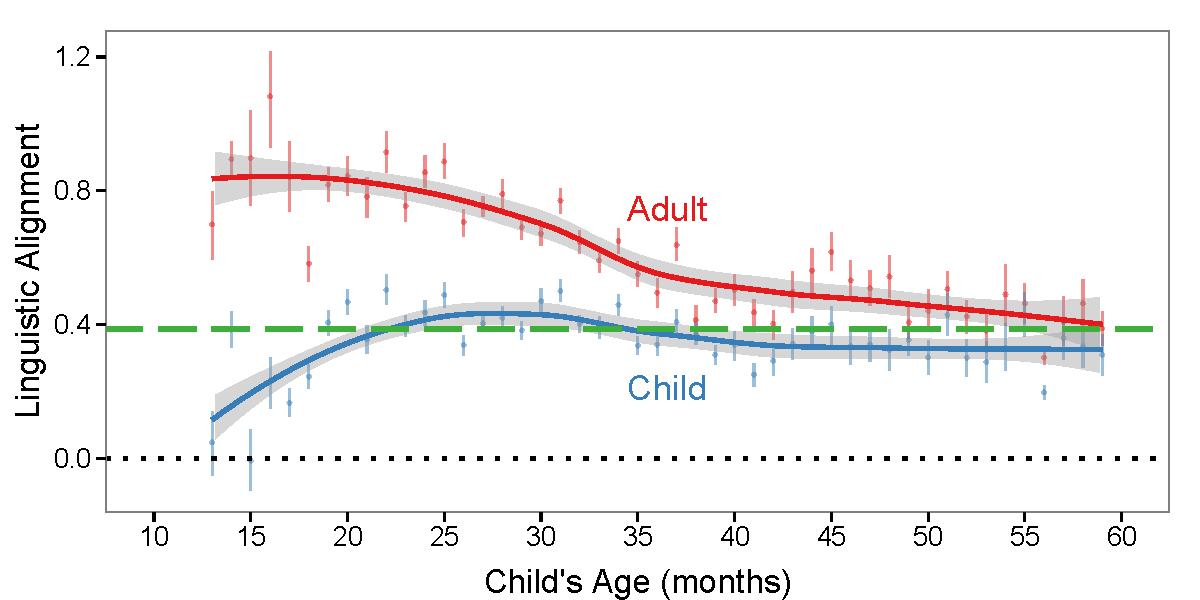
\includegraphics[width=.95\textwidth]{figures/all_childes.pdf}}
	\caption{\label{fig:all_childes} }
\end{figure*}

\section{General Discussion}




desirable difficulties, goldolicks

People have proposed that the answer is in the input. \cite<c.f.>{mcmurray2007}

But changes in competencies suggest that different things need to be scaffolded at different times. Proposal: all input is not created equal, easier input earlier (elman, caitlin)

linguistic alignment as one relatively easy measure. Function vs. Content,



\section{Acknowledgments}

We are grateful to all of the members of the Language and Cognition Lab for their feedback on this project. This work was supported by NIH NRSA F32HD075577 to DY and STUFF FOR GABE AND MIKE.

\bibliographystyle{myapacite}

\setlength{\bibleftmargin}{.125in}
\setlength{\bibindent}{-\bibleftmargin}

\bibliography{alignment}


\end{document}
